
%(BEGIN_QUESTION)
% Copyright 2006, Tony R. Kuphaldt, released under the Creative Commons Attribution License (v 1.0)
% This means you may do almost anything with this work of mine, so long as you give me proper credit

Graph the output of this proportional-only controller, assuming a gain ($K_p$) value of 0.5, a bias value of 40\%, and a control action that is reverse-acting:

$$\includegraphics[width=15.5cm]{i01485x01.eps}$$

\vskip 20pt \vbox{\hrule \hbox{\strut \vrule{} {\bf Suggestions for Socratic discussion} \vrule} \hrule}

\begin{itemize}
\item{} Identify points on the trend where the PV exhibits a positive rate of change. 
\item{} Identify points on the trend where the PV exhibits a negative rate of change. 
\item{} Identify points on the trend where the PV exhibits zero change. 
\item{} How would the output signal trend be altered if the {\it gain} of this controller were decreased?
\item{} How would the output signal trend be altered if the {\it bias} of this controller were decreased?
\item{} How would the output signal trend be altered if the {\it action} of this controller were switched from reverse to direct?
\end{itemize}

\underbar{file i01485}
%(END_QUESTION)





%(BEGIN_ANSWER)

$$\includegraphics[width=15.5cm]{i01485x02.eps}$$

%(END_ANSWER)





%(BEGIN_NOTES)

With a gain of 0.5, the proportional band value will be 200\%.

$$m = 0.5(\hbox{SP} - \hbox{PV}) + 40$$

% No blank lines allowed between lines of an \halign structure!
% I use comments (%) instead, so that TeX doesn't choke.

$$\vbox{\offinterlineskip
\halign{\strut
\vrule \quad\hfil # \ \hfil & 
\vrule \quad\hfil # \ \hfil & 
\vrule \quad\hfil # \ \hfil \vrule \cr
\noalign{\hrule}
%
% First row
{\bf PV} & {\bf SP} & {\bf Output} \cr
%
\noalign{\hrule}
%
% Another row
50\% & 45\% & 37.5\% \cr
%
\noalign{\hrule}
%
% Another row
70\% & 45\% & 27.5\% \cr
%
\noalign{\hrule}
%
% Another row
70\% & 55\% & 32.5\% \cr
%
\noalign{\hrule}
%
% Another row
50\% & 40\% & 35\% \cr
%
\noalign{\hrule}
} % End of \halign 
}$$ % End of \vbox


%INDEX% Control, proportional: graphing controller response

%(END_NOTES)


